\documentclass[11pt]{article}
\usepackage[left=2.2cm,right=2.2cm,top=2.3cm,bottom=2.3cm]{geometry}
\usepackage[T1]{fontenc}
\usepackage[utf8]{inputenc}
\usepackage{lmodern}
\usepackage{amsmath}
\usepackage{booktabs}
\usepackage{tabularx}
\usepackage{longtable}
\usepackage{array}
\usepackage{xcolor}
\usepackage{pdflscape}
\usepackage{caption}
\usepackage{tikz}
\usepackage[hidelinks]{hyperref}
\usetikzlibrary{arrows.meta, positioning, calc, fit, backgrounds}

\setlength{\parindent}{0mm}
\setlength{\parskip}{2mm}
\renewcommand{\arraystretch}{1.25}
\newcolumntype{L}{>{\raggedright\arraybackslash}X}
\newcolumntype{P}[1]{>{\raggedright\arraybackslash}p{#1}}

% Variable and POU names, typewriter, breakable at dots
\DeclareUrlCommand\var{\urlstyle{tt}}
% Code expressions with spaces
\newcommand{\code}[1]{\texttt{#1}}
% Deviation from the functional description / open issue, numbered in Section 7
\newcommand{\dev}[1]{\textsuperscript{\textcolor{red}{\textbf{D#1}}}}

% Diagram styles after Cooling [COO] Fig. 7.1 and 7.8: software machines (SM) as numbered
% boxes on a light background, external items as plain boxes, data items written on the arrows.
\tikzset{
  sm/.style={draw, rectangle, fill=yellow!12, align=center, inner sep=4pt,
             minimum height=12mm, font=\small},
  ext/.style={draw, rectangle, fill=gray!12, align=center, inner sep=4pt,
              minimum height=10mm, font=\small},
  extoff/.style={ext, dashed, text=gray, draw=gray},
  store/.style={draw=none, align=center, inner sep=3pt, font=\small,
                append after command={
                  [draw] (\tikzlastnode.north west) -- (\tikzlastnode.north east)
                  (\tikzlastnode.south west) -- (\tikzlastnode.south east)}},
  flow/.style={-{Stealth[length=2.2mm]}, thick},
  fb/.style={flow, densely dashed},
  lab/.style={font=\scriptsize\ttfamily, align=center, fill=white, inner sep=1pt},
  num/.style={font=\scriptsize\bfseries},
  state/.style={draw, rectangle, rounded corners=2pt, fill=yellow!12, minimum width=24mm,
                minimum height=9mm, align=center, font=\small},
}

\title{CAS (Heimdall) -- program design\\[1mm]
\large Inlet pump: configuration, commands, prerequisites and dataflow}
\author{Sigurd R. Brekk}
\date{\today}

\begin{document}
\maketitle

\section{Purpose}

This document shows how the Heimdall PLC program starts and runs an inlet pump.
It answers four questions:
\begin{enumerate}
  \item which configuration values must be set before an inlet pump can start (Section~\ref{sec:config});
  \item which commands start, stop and reset it (Section~\ref{sec:commands});
  \item which other systems must be available or running (Section~\ref{sec:prereq});
  \item how a value travels through the program, from the Modbus word read from the remote I/O to
        the speed setpoint written to the Framo controller (Section~\ref{sec:dataflow}).
\end{enumerate}
Section~\ref{sec:dev} lists where the program differs from the functional description [FD] and
other issues found while tracing the dataflow.

The program was read on 2026-10-15 from the CODESYS project \var{heimdall-plc}, branch
\var{inletControl}, application \var{PFC200_Sim}, after the merge with the outlet valve work.

\subsection*{Sources}
\begin{tabularx}{\textwidth}{@{}lL@{}}
\toprule
ID & Document \\
\midrule
{[COO]} & J.~Cooling, \emph{Software Engineering for Real-Time Systems} (The Complete Edition),
          Packt, 2020. \S4.6.2 materials flow model, \S7.2.1 context diagrams, \S7.2.3 state
          transition diagrams, \S7.2.4 functional and data flow diagrams, \S14.3.3 functional
          diagram description. \\
{[FD]}  & P-15169-CAS-FD-01 Funksjonsbeskrivelse CAS, rev.~B, 13.05.26. \S3.2.1 Vanninntak,
          \S3.2.2 Regulering av vann-nivå i merden, \S3.2.4 Oksygentilførsel. \\
{[DES]} & CAS (Heimdall) -- design basis for control (\emph{System Modelling/CAS design basis.tex}). \\
{[PLC]} & CODESYS project heimdall-plc, branch inletControl, application PFC200\_Sim (read
          2026-10-15). \\
\bottomrule
\end{tabularx}

\section{Notation}
\label{sec:notation}

The diagrams follow Cooling's functionally structured diagrams [COO \S7.2].
\begin{itemize}
  \item A \textbf{context diagram} [COO \S7.2.1, Fig.~7.1] shows the PLC software as one black
        box and the external items it exchanges data with. It defines every device the software
        talks to and every signal it must handle.
  \item A \textbf{functional flow diagram} (FFD) [COO \S7.2.4, Fig.~7.8] shows the processing as a
        flow of material, here data, through \emph{software machines} (SM). Each SM is a
        self-contained unit with one clear function; its outputs are the result of processing its
        inputs. The underlying model is the materials flow model [COO \S4.6.2]: a value enters on
        the left and is worked on by one SM after the other, like a work piece on a production
        line.
  \item Since the PLC runs the SMs in sequential code, only one SM is active at a time and the
        order matters. The FFD is therefore accompanied by an \textbf{execution sequence}
        [COO Fig.~7.10] that names the code unit (task, program, function block) running each SM.
  \item The behaviour over time of the Framo pump state is shown in a \textbf{state transition
        diagram} [COO \S7.2.3, Fig.~7.6].
\end{itemize}

In CODESYS terms an SM is a program (PRG), a function block (FB) instance or a method. Its
\emph{in parameters} are the variables it reads (VAR\_INPUT or VAR\_IN\_OUT), its \emph{out
parameters} the variables it writes. Variable names are given in full from the global variable
list, e.g.\ \var{GVLMain.Inlet[i].InletPump.State}; \var{i} = 0, 1, 2 is the inlet (inlet 1, 2, 3)
and \var{n} = \var{i}+1 numbers the Framo data sources \var{Framo_1..3}.

Symbols used in the diagrams:

\begin{center}
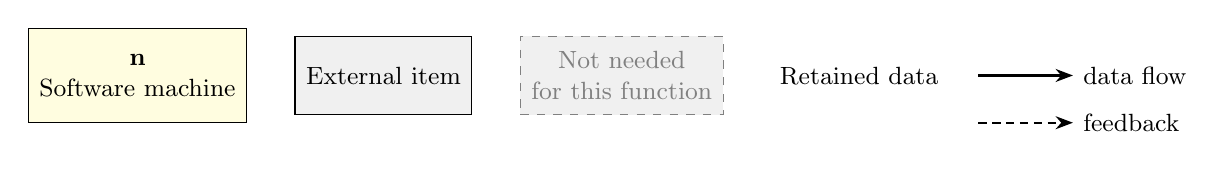
\begin{tikzpicture}[node distance=6mm]
  \node[sm] (a) {\textbf{n}\\Software machine};
  \node[ext, right=of a] (b) {External item};
  \node[extoff, right=of b] (c) {Not needed\\for this function};
  \node[store, right=of c] (d) {Retained data};
  \draw[flow] ($(d.east)+(4mm,0)$) -- ++(12mm,0) node[right, font=\small] {data flow};
  \draw[fb] ($(d.east)+(4mm,-6mm)$) -- ++(12mm,0) node[right, font=\small] {feedback};
\end{tikzpicture}
\end{center}

% ---------------------------------------------------------------------------------------------
\section{Context diagram}
\label{sec:context}

Figure~\ref{fig:context} shows the PLC software and its surroundings as far as the inlet pumps are
concerned. Table~\ref{tab:context} gives the interface of each external item.

\begin{figure}[htbp]
\centering
\resizebox{\linewidth}{!}{%
\begin{tikzpicture}[node distance=10mm and 36mm]
  \node[sm, minimum width=46mm, minimum height=34mm, font=\normalsize] (plc)
       {\textbf{Heimdall PLC software}\\[1mm]\small PFC200 750-8212\\\small 10.1.2.41\\[1mm]
        \small application \var{PFC200_Sim}};

  \node[ext, left=of plc, yshift=10mm, minimum width=30mm] (irio)
       {\textbf{InletRIO 1--3}\\\footnotesize 750-455, Modbus TCP};
  \node[extoff, left=of plc, yshift=-10mm, minimum width=30mm] (crio)
       {\textbf{CommonRIO}\\\footnotesize Orbit 864, O$_2$ valves};
  \node[ext, right=of plc, minimum width=30mm] (framo)
       {\textbf{Framo local}\\\textbf{controller 1--3}\\\footnotesize OPC UA server};
  \node[ext, above=of plc, minimum width=40mm] (hmi)
       {\textbf{Operator (HMI)}\\\footnotesize OPC UA client to the PLC};
  \node[store, below=of plc, minimum width=40mm] (ret)
       {\textbf{GVLRetain}\\\footnotesize persistent memory};

  \draw[flow] (irio) -- node[lab, above] {level inside,\\outside} (plc.west |- irio);
  \draw[flow, gray] (crio) -- node[lab, below, text=gray] {O$_2$ (not used)} (plc.west |- crio);
  \draw[flow] ([yshift=4mm]plc.east) -- node[lab, above] {Start, Stop, Reset,\\VelocitySetpoint} ([yshift=4mm]framo.west);
  \draw[flow] ([yshift=-4mm]framo.west) -- node[lab, below] {PumpState*, MotorVelocity,\\alarms, HeartbeatToggle} ([yshift=-4mm]plc.east);
  \draw[flow] ([xshift=-8mm]hmi.south) -- node[lab, left] {commands,\\configuration} ([xshift=-8mm]plc.north);
  \draw[flow] ([xshift=8mm]plc.north) -- node[lab, right] {status,\\alarms} ([xshift=8mm]hmi.south);
  \draw[flow, <->] (plc) -- node[lab, right] {configuration} (ret);
\end{tikzpicture}}
\caption{Context diagram of the inlet pump function [COO Fig.~7.1]. The CommonRIO carries the
oxygen sensors and valves; the inlet pump does not need it.}
\label{fig:context}
\end{figure}

\begin{table}[htbp]
\centering\small
\caption{External items of the inlet pump function.}
\label{tab:context}
\begin{tabularx}{\textwidth}{@{}P{24mm}P{30mm}P{37mm}L@{}}
\toprule
External item & Link & PLC code unit & Data \\
\midrule
InletRIO 1--3 & Modbus TCP, FC23, read words 0--25, write words 0--20, every 60~ms &
  \var{InletRIO[i]} in \var{PRG.IO_Processing} &
  In: level inside (word 0), level outside (word 1), oxy pump and oxynator pressure (words 2, 3),
  digital inputs (words 4, 5). Out: reset of field power (word 0 bit 0). \\
Framo local controller 1--3 & OPC UA, data sources \var{Framo_1..3} in the \var{DatasourcesManager} &
  \var{PRG.FramoDataProcessing}, \var{Datasources_PRG} &
  In: pump state, motor values, alarms, heartbeat [FD Tabell~6]. Out: \var{Start},
  \var{Stop}, \var{Reset}, \var{SpeedSetpoint}. \\
Operator (HMI) & OPC UA server of the PLC (Symbol Configuration: \var{GVLMain}, \var{GVLIO}) &
  -- & Writes commands and configuration in \var{GVLMain}; reads status and alarms. \\
GVLRetain & persistent variables & \var{Main.UpdateRetain} &
  Configuration copied to \var{GVLMain} in the first cycle, and back on every change. \\
CommonRIO & Modbus TCP and Modbus RTU (750-652) & \var{CommonRIO}, \var{IO_Processing_RTU} &
  Oxygen sensors and valves. Not needed to start or run an inlet pump. \\
\bottomrule
\end{tabularx}
\end{table}

% ---------------------------------------------------------------------------------------------
\section{Tasks and execution sequence}
\label{sec:tasks}

The SMs run in three tasks (Task Configuration of \var{PFC200_Sim}). Within a task the programs run
in the order listed, and within \var{PRG.Main} the function blocks run in the order they are
called. Figure~\ref{fig:exec} is the execution sequence in the outline form of [COO Fig.~7.10].

\begin{figure}[htbp]
\centering
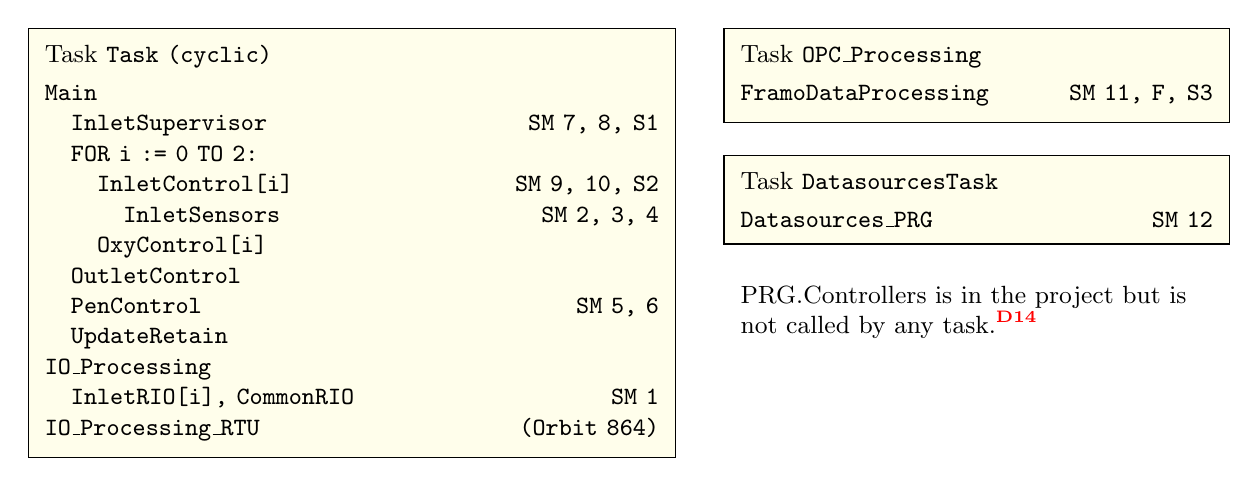
\begin{tikzpicture}
  \node[draw, fill=yellow!8, align=left, font=\small\ttfamily, inner sep=6pt, text width=78mm] (t1) {%
  \textbf{\normalfont Task \texttt{Task}} (cyclic)\\[1mm]
  Main\\
  \quad InletSupervisor \hfill SM 7, 8, S1\\
  \quad FOR i := 0 TO 2:\\
  \quad\quad InletControl[i] \hfill SM 9, 10, S2\\
  \quad\quad\quad InletSensors \hfill SM 2, 3, 4\\
  \quad\quad OxyControl[i]\\
  \quad OutletControl\\
  \quad PenControl \hfill SM 5, 6\\
  \quad UpdateRetain\\
  IO\_Processing\\
  \quad InletRIO[i], CommonRIO \hfill SM 1\\
  IO\_Processing\_RTU \hfill (Orbit 864)};
  \node[draw, fill=yellow!8, align=left, font=\small\ttfamily, inner sep=6pt, text width=60mm,
        right=6mm of t1.north east, anchor=north west] (t2) {%
  \textbf{\normalfont Task \texttt{OPC\_Processing}}\\[1mm]
  FramoDataProcessing \hfill SM 11, F, S3};
  \node[draw, fill=yellow!8, align=left, font=\small\ttfamily, inner sep=6pt, text width=60mm,
        below=4mm of t2] (t3) {%
  \textbf{\normalfont Task \texttt{DatasourcesTask}}\\[1mm]
  Datasources\_PRG \hfill SM 12};
  \node[align=left, font=\small, text width=60mm, below=4mm of t3] {%
  \var{PRG.Controllers} is in the project but is not called by any task.\dev{14}};
\end{tikzpicture}
\caption{Execution sequence [COO Fig.~7.10]. SM numbers refer to Figure~\ref{fig:ffd} and
Table~\ref{tab:dataflow}; S1--S3 and F to Figure~\ref{fig:start}.}
\label{fig:exec}
\end{figure}

\textbf{Consequence for the timing.} \var{IO_Processing} runs after \var{Main}, and
\var{InletSupervisor} runs before \var{PenControl}. A level word read in cycle $k$ is therefore
scaled and averaged in cycle $k+1$ and reaches the level controller in cycle $k+2$. The speed
setpoint is then handed to \var{FramoDataProcessing} in the next run of
\var{OPC_Processing}, and the OPC UA client sends it with its own publishing interval. Together
with the 60~ms Modbus poll this is some tenths of a second, small next to the 2~s dead time of the
level loop [DES \S7].

% ---------------------------------------------------------------------------------------------
\section{Starting an inlet pump}
\label{sec:start}

\subsection{Pump state}
\label{sec:state}

The Framo local controller owns the pump state. It publishes one Boolean per state
(\var{PumpStateAvailable}, \var{PumpStateStart}, \ldots); \var{FramoDataProcessing} turns these into
the enumeration \var{GVLMain.Inlet[i].InletPump.State} (\var{ENUM.InletPumpState}). The PLC only
asks for transitions with \var{Start}, \var{Stop} and \var{Reset}. Figure~\ref{fig:std} is the state
transition diagram as described in [FD Tabell~5]; Table~\ref{tab:states} shows what the PLC does in
each state (\var{InletControl.InletPumpControl}).

\begin{figure}[htbp]
\centering
\resizebox{\linewidth}{!}{%
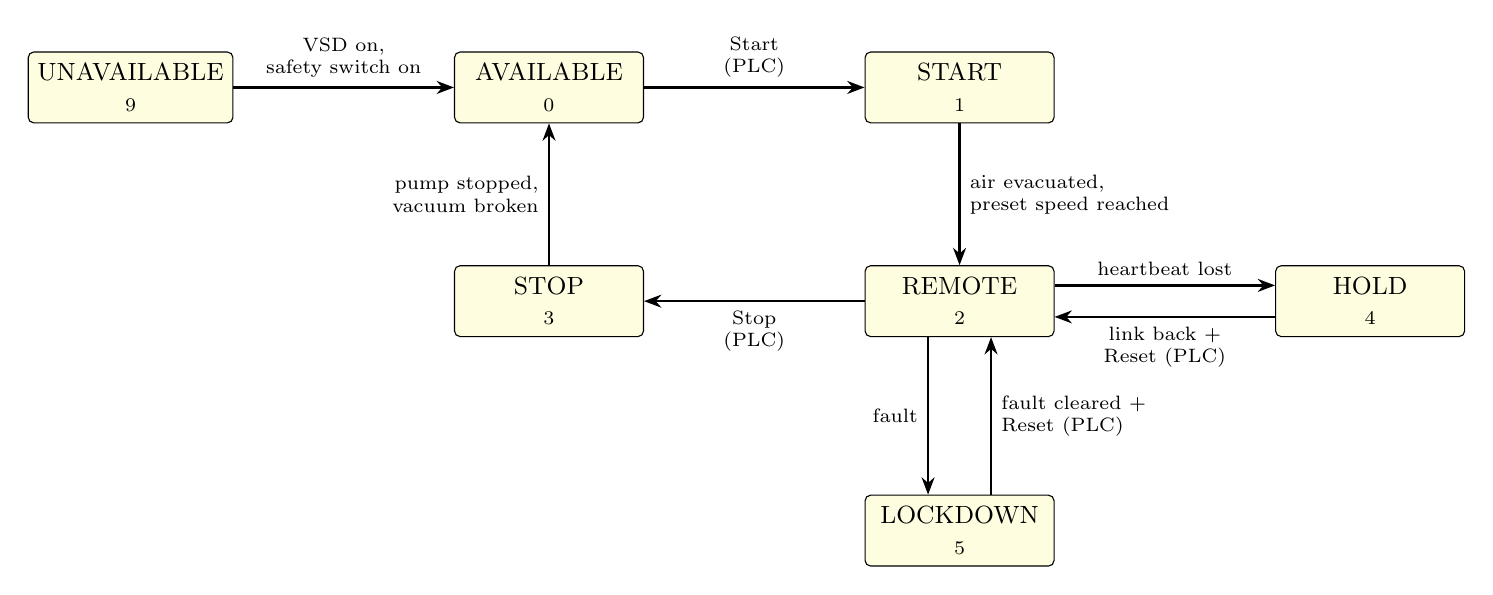
\begin{tikzpicture}[node distance=12mm and 28mm, every edge quotes/.style={font=\scriptsize}]
  \node[state] (una) {UNAVAILABLE\\\scriptsize 9};
  \node[state, right=of una] (ava) {AVAILABLE\\\scriptsize 0};
  \node[state, right=of ava] (sta) {START\\\scriptsize 1};
  \node[state, below=18mm of sta] (rem) {REMOTE\\\scriptsize 2};
  \node[state, below=18mm of ava] (stp) {STOP\\\scriptsize 3};
  \node[state, right=of rem] (hol) {HOLD\\\scriptsize 4};
  \node[state, below=20mm of rem] (loc) {LOCKDOWN\\\scriptsize 5};

  \draw[flow] (una) -- node[above, font=\scriptsize, align=center] {VSD on,\\safety switch on} (ava);
  \draw[flow] (ava) -- node[above, font=\scriptsize, align=center] {\var{Start}\\(PLC)} (sta);
  \draw[flow] (sta) -- node[right, font=\scriptsize, align=left] {air evacuated,\\preset speed reached} (rem);
  \draw[flow] (rem) -- node[below, font=\scriptsize, align=center] {\var{Stop}\\(PLC)} (stp);
  \draw[flow] (stp) -- node[left, font=\scriptsize, align=right] {pump stopped,\\vacuum broken} (ava);
  \draw[flow] ([yshift=2mm]rem.east) -- node[above, font=\scriptsize] {heartbeat lost} ([yshift=2mm]hol.west);
  \draw[flow] ([yshift=-2mm]hol.west) -- node[below, font=\scriptsize, align=center] {link back +\\\var{Reset} (PLC)} ([yshift=-2mm]rem.east);
  \draw[flow] ([xshift=-4mm]rem.south) -- node[left, font=\scriptsize] {fault} ([xshift=-4mm]loc.north);
  \draw[flow] ([xshift=4mm]loc.north) -- node[right, font=\scriptsize, align=left] {fault cleared +\\\var{Reset} (PLC)} ([xshift=4mm]rem.south);
\end{tikzpicture}}
\caption{State transition diagram of the Framo inlet pump [FD Tabell~5], [COO \S7.2.3]. Numbers
are the values of \texttt{ENUM.InletPumpState}. Transitions not described in [FD] (e.g.\ from
LOCKDOWN after \texttt{Reset} when the pump has stopped) are set by the Framo controller.}
\label{fig:std}
\end{figure}

\begin{table}[htbp]
\centering\small
\caption{PLC action per pump state (\texttt{InletControl.InletPumpControl}).}
\label{tab:states}
\begin{tabularx}{\textwidth}{@{}lP{40mm}cccL@{}}
\toprule
State & \var{Output.VelocitySetpoint} & Start allowed & Running & In LIC01 & Comment \\
\midrule
UNAVAILABLE & 0 & no & no & no & Also shown while the Framo link is down (no heartbeat answer).\dev{9} \\
AVAILABLE & \var{Input.MotorVelocity} & yes & no & no & Setpoint follows the actual speed, as [FD] asks. \\
START & \var{Input.MotorVelocity} & yes & yes & yes & LIC01 tracks the mean speed of the starting pumps (SM~7). \\
REMOTE & \var{InletPumpSpeedSetpoint} (LIC01 output in auto, \var{Command.Setpoint} in manual) & yes & yes & yes & The only state in which the PLC sets the speed. \\
HOLD & \var{Input.MotorVelocity} & yes & yes\textsuperscript{*} & no\textsuperscript{*} & Framo runs a preset speed. LIC01 is frozen until the pump is back in REMOTE.\dev{3} \\
STOP & 0 & no & yes & yes & \\
LOCKDOWN & 0 & no & no & no & Needs \var{Reset}. \\
\bottomrule
\multicolumn{6}{@{}p{\textwidth}@{}}{\footnotesize\textsuperscript{*} The local variable
\var{Running} is set TRUE in the HOLD branch, but \var{Status.EnableLevelControl} is computed
before the CASE from the states START, REMOTE and STOP only. \code{Start allowed} =
\var{StartAvailable}; \code{In LIC01} = \var{Status.EnableLevelControl} with the pump in auto.}
\end{tabularx}
\end{table}

\subsection{Other systems that must be available or running}
\label{sec:prereq}

Table~\ref{tab:prereq} lists what must be in place before \var{Start} reaches the pump and the
level controller can take over. Only the first four rows are needed for the pump to start. The
rest are needed for level control.

\begin{table}[htbp]
\centering\small
\caption{Prerequisites for starting an inlet pump.}
\label{tab:prereq}
\begin{tabularx}{\textwidth}{@{}P{38mm}LP{40mm}@{}}
\toprule
System & What must hold & Where the PLC sees it \\
\midrule
Framo local controller $n$ & Powered, VSD on, safety switch on, no emergency stop, no fault;
  vacuum system ready (handled by the local controller). Pump state AVAILABLE. &
  \code{Inlet[i].InletPump.State = Available} \\
OPC UA link to Framo $n$ & Data source \var{Framo_n} connected, so that commands are written and
  the state is read; Framo answers the heartbeat. Without it the PLC shows the pump UNAVAILABLE and
  sends no Start.\dev{9} &
  \var{Inlet[i].InletPump.Status.CommunicationOK} \\
PLC application & Running, with the tasks \var{Task}, \var{OPC_Processing} and
  \var{DatasourcesTask}. & -- \\
Operator (HMI) & Connected to the PLC's OPC UA server to write the commands. & -- \\
\midrule
InletRIO $i$ & Connected (\var{GVLIO.InletRIO[i].Status.CommOK}); otherwise the level words are not
  updated. Not an interlock for the start. & \var{InletRIO[i].Status.CommOK} \\
Level transmitters LT inside/outside & At least one valid pair: both transmitters of an inlet
  4--20~mA healthy (status bits 1..0 $=$ 00) and enabled, and the pair enabled. Without one, LIC01
  runs the pumps at \var{SafeOutput} and raises \emph{LevelMeasurementLost}. Not an interlock for
  the start. & \var{Pen.Status.LevelControlOK} \\
\midrule
Oxygen system, outlet valve, CommonRIO & Not needed. In [FD] the oxygen system depends on the
  inlet pump, not the other way round: the oxy pump runs only when the inlet pump on the same
  line runs [FD \S3.2.4]. & -- \\
\bottomrule
\end{tabularx}
\end{table}

\subsection{Configuration}
\label{sec:config}

Table~\ref{tab:config} lists the configuration values the inlet pump function uses. All but the
data source endpoints live in \var{GVLMain}, are written from the HMI and are kept in
\var{GVLRetain} by \var{Main.UpdateRetain}. Defaults are those in \var{GVL.ConfigValues} of
\var{PFC200_Sim}, applied on a fresh download.

\begin{table}[htbp]
\centering\small
\caption{Configuration for the inlet pump function. \emph{Needed for}: S = pump start,
L = level control.}
\label{tab:config}
\begin{tabularx}{\textwidth}{@{}P{58mm}P{30mm}cL@{}}
\toprule
Variable & Default & For & Meaning, and what happens if it is wrong \\
\midrule
Data sources \var{Framo_1..3} (DatasourcesManager) & per project & S &
  OPC UA endpoint of each Framo controller. Wrong: no commands reach the pump. \\
\var{InletRIOConfig[i].Enabled} & TRUE & L & Connects the Modbus TCP master. \\
\var{InletRIOConfig[i].IP}, \var{.Port} & 10.1.2.101, 5121--5123 (simulator) & L &
  Address of InletRIO $i$. IP 0 or port 0 raises \emph{MissingIPaddress}. \\
\var{Inlet[i].Input.LevelInsidePen.Config.Enable} & TRUE & L &
  Transmitter in use; disabled, its pair drops out. \\
\var{Inlet[i].Input.LevelInsidePen.Config.MinValue}, \var{.MaxValue} & 0.0, 2.0~m & L &
  Range for 4 and 20~mA. \\
\var{Inlet[i].Input.LevelInsidePen.Config.QualityEnabled} & TRUE & L &
  Quality alarm on a bad transmitter (after \var{QualityDelay}, 1~s). \\
\var{Inlet[i].Input.LevelInsidePen.Config.FilterFc} & 0.05~Hz & -- &
  Display smoothing only; not in the control path. \\
\var{Inlet[i].Input.LevelOutsidePen.Config.*} & as inside & L & Same for the outside transmitter. \\
\var{Inlet[i].Input.PenOverHeight.Config.Enable} & TRUE & L &
  The inlet's level pair is used in LIC01's process value. \\
\var{Inlet[i].Input.PenOverHeight.Config.FilterFc} & 0.05~Hz & L &
  Cut-off of the pair's Butterworth2 low-pass; 0 turns it off. \\
\var{PenConfig.LevelController.Kp} & 450~rpm/m & L & Gain of LIC01. \\
\var{PenConfig.LevelController.Ti} & 60~s\dev{11} & L & Integral time. \\
\var{PenConfig.LevelController.Td} & 0~s & L & Derivative time (0 = PI). \\
\var{PenConfig.LevelController.MinOutput}, \var{.MaxOutput} & 40, 130~rpm & L &
  Speed range of the pumps [FD Tabell~8]; also the PID's output limits. \\
\var{PenConfig.LevelController.SafeOutput} & 60~rpm & L &
  Pump speed while no valid level pair is left. \\
\var{InletConfig[i].HeartbeatInterval}, \var{.HeartbeatTimeout} & 1~s, 5~s & S &
  Framo heartbeat: the PLC sets the shared bit 1~s after Framo cleared it; alarm when Framo has
  not cleared it for 5~s. \\
\var{InletConfig[i].StartupTime}, \var{.ShutdownTime} & 30~s, 30~s & S &
  Longest time from Start (Stop) until Framo reports START (STOP); then the start-up (stop) timeout
  alarm.\dev{8} \\
\bottomrule
\end{tabularx}
\end{table}

\subsection{Commands}
\label{sec:commands}

The commands are variables in \var{GVLMain} that the HMI sets. Commands marked \emph{pulse} are
reset by the PLC once acted on. Table~\ref{tab:commands} gives the commands; the steps below give
the order.

\textbf{Automatic start of the pen (normal operation).}
\begin{enumerate}
  \item Put each pump that shall run in auto: \var{Inlet[i].InletPump.Command.Auto} (default: auto).
  \item Set the level setpoint \var{Pen.Command.LevelSetpoint} [m]; it is retained.\dev{13}
  \item Leave LIC01 in auto (\var{LevelController.Command.Manual} = FALSE, default).
  \item Give \var{Pen.Command.Start}. Every pump in auto gets \var{Start}; while a pump is in START,
        LIC01 follows its speed, and when the first pump reaches REMOTE LIC01 takes over
        bumplessly.
  \item \var{Pen.Command.Stop} stops every pump in auto.
\end{enumerate}

\textbf{Manual start of one pump.}
\begin{enumerate}
  \item \var{Inlet[i].InletPump.Command.Manual}; the pump leaves level control.
  \item Set the speed \var{Inlet[i].InletPump.Command.Setpoint} [rpm]; used in REMOTE.
  \item \var{Inlet[i].InletPump.Command.Start}; stop with \var{Inlet[i].InletPump.Command.Stop}.
\end{enumerate}

\begin{table}[htbp]
\centering\small
\caption{Commands for the inlet pumps.}
\label{tab:commands}
\begin{tabularx}{\textwidth}{@{}P{58mm}P{18mm}L@{}}
\toprule
Command & Type & Effect \\
\midrule
\var{Pen.Command.Start} & pulse & Latches \var{PenStart} in \var{InletSupervisor}; every pump in auto
  gets \var{Inlet[i].Command.AutoStartInletPump}. Reset by the PLC when a pump runs. \\
\var{Pen.Command.Stop} & pulse & Clears \var{PenStart}; every pump in auto gets
  \var{AutoStopInletPump}. \\
\var{Pen.Command.LevelSetpoint} & value [m] & Setpoint of LIC01 (overheight inside the pen).
  [FD] gives it in cm. \\
\var{Inlet[i].InletPump.Command.Manual} / \var{.Auto} & pulse & Sets / clears
  \var{InletPump.Status.Manual}. \\
\var{Inlet[i].InletPump.Command.Start} / \var{.Stop} & pulse & Start or stop in manual. \\
\var{Inlet[i].InletPump.Command.Setpoint} & value [rpm] & Speed in manual, sent in REMOTE. \\
\var{Inlet[i].InletPump.Command.Reset} & level & Sent to Framo as \var{Reset} (HOLD, LOCKDOWN). \\
\var{LevelController.Command.Manual} / \var{.Auto} & level / pulse & LIC01 manual or auto. \\
\var{LevelController.Command.ManualOutput} & value [rpm] & LIC01 output in manual. \\
\bottomrule
\end{tabularx}
\end{table}

\subsection{Start command path}

Figure~\ref{fig:start} follows the start command from the HMI to the Framo controller and the
pump state back. Table~\ref{tab:startflow} names the variables.

\begin{figure}[htbp]
\centering
\resizebox{\linewidth}{!}{%
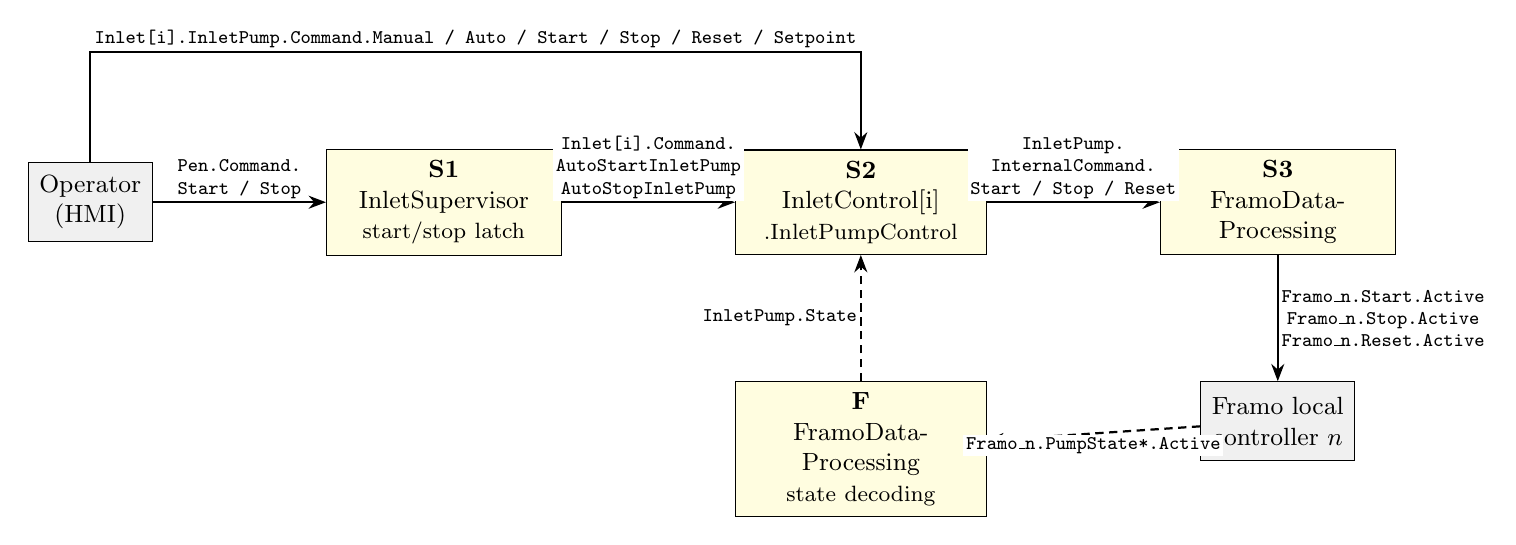
\begin{tikzpicture}[node distance=9mm and 22mm]
  \node[ext] (hmi) {Operator\\(HMI)};
  \node[sm, right=of hmi, text width=27mm] (s1) {\textbf{S1}\\InletSupervisor\\\footnotesize start/stop latch};
  \node[sm, right=of s1, text width=29mm] (s2) {\textbf{S2}\\InletControl[i]\\\footnotesize .InletPumpControl};
  \node[sm, right=of s2, text width=27mm] (s3) {\textbf{S3}\\FramoData-\\Processing};
  \node[ext, below=16mm of s3] (fr) {Framo local\\controller $n$};
  \node[sm, below=16mm of s2, text width=29mm] (f) {\textbf{F}\\FramoData-\\Processing\\\footnotesize state decoding};

  \draw[flow] (hmi) -- node[lab, above] {Pen.Command.\\Start / Stop} (s1);
  \draw[flow] (s1) -- node[lab, above] {Inlet[i].Command.\\AutoStartInletPump\\AutoStopInletPump} (s2);
  \draw[flow] (s2) -- node[lab, above] {InletPump.\\InternalCommand.\\Start / Stop / Reset} (s3);
  \draw[flow] (s3) -- node[lab, right] {Framo\_n.Start.Active\\Framo\_n.Stop.Active\\Framo\_n.Reset.Active} (fr);
  \draw[fb] (fr) -- node[lab, below] {Framo\_n.PumpState*.Active} (f);
  \draw[fb] (f) -- node[lab, left] {InletPump.State} (s2);
  \draw[flow] (hmi.north) -- ++(0,14mm) -| node[lab, pos=0.25, above] {Inlet[i].InletPump.Command.Manual / Auto / Start / Stop / Reset / Setpoint}
        (s2.north);
\end{tikzpicture}}
\caption{FFD of the start command [COO Fig.~7.8]. The manual commands enter at S2.}
\label{fig:start}
\end{figure}

\begin{table}[htbp]
\centering\small
\caption{Start command dataflow.}
\label{tab:startflow}
\begin{tabularx}{\textwidth}{@{}cP{36mm}P{44mm}L@{}}
\toprule
SM & Code unit & Reads & Operation and writes \\
\midrule
S1 & \var{InletSupervisor} (body) & \var{Pen.Command.Start}, \var{Pen.Command.Stop},
  \var{Inlet[i].InletPump.Status.Manual} &
  \code{PenStart := (PenStart OR Start) AND NOT Stop}. For each pump not in manual:
  \code{Inlet[i].Command.AutoStartInletPump := PenStart},
  \code{AutoStopInletPump := NOT PenStart}. \\
S2 & \var{InletControl[i].InletPumpControl} & \var{AutoStartInletPump}, \var{AutoStopInletPump}
  (auto) or \var{InletPump.Command.Start/Stop} (manual); \var{InletPump.State} &
  \var{StartPump} latches the start until a stop; \var{StopRequest} = stop command.
  \code{InletPump.Output.Start := StartPump AND StartAvailable}. The body copies to
  \var{InletPump.InternalCommand.Start}, \code{.Stop := StopRequest},
  \code{.Reset := Command.Reset}. \\
S3 & \var{FramoDataProcessing} & \var{Inlet[i].InletPump.InternalCommand.*} &
  \var{Framo_n.Start.Active}, \var{Framo_n.Stop.Active}, \var{Framo_n.Reset.Active}; the Framo
  controller acts on the rising edge. \\
F & \var{FramoDataProcessing} & \var{Framo_n.PumpStateUnavailable.Active} \ldots
  \var{PumpStateLockdown.Active} &
  While \var{Inlet[i].InletPump.Status.CommunicationOK} (set by \var{InletControl} from the
  heartbeat): the first TRUE flag sets \var{Inlet[i].InletPump.State}. Otherwise
  \var{State := Unavailable}.\dev{9} \\
\bottomrule
\end{tabularx}
\end{table}

% ---------------------------------------------------------------------------------------------
\begin{landscape}
\section{Dataflow: from level transmitter to pump speed}
\label{sec:dataflow}

Figure~\ref{fig:ffd} is the functional flow diagram of the level loop, the main dataflow of the
inlet pump: the two level words read from InletRIO $i$ are scaled, their difference (the inlet's
level pair) is filtered, the valid pairs are averaged over the inlets, the result is compared with
the setpoint in LIC01, and the controller output is sent as the speed setpoint to
every pump in level control. Table~\ref{tab:dataflow} names, for every SM, the variables it reads,
what it does with them and the variables it writes.

\begin{center}
\resizebox{\linewidth}{!}{%
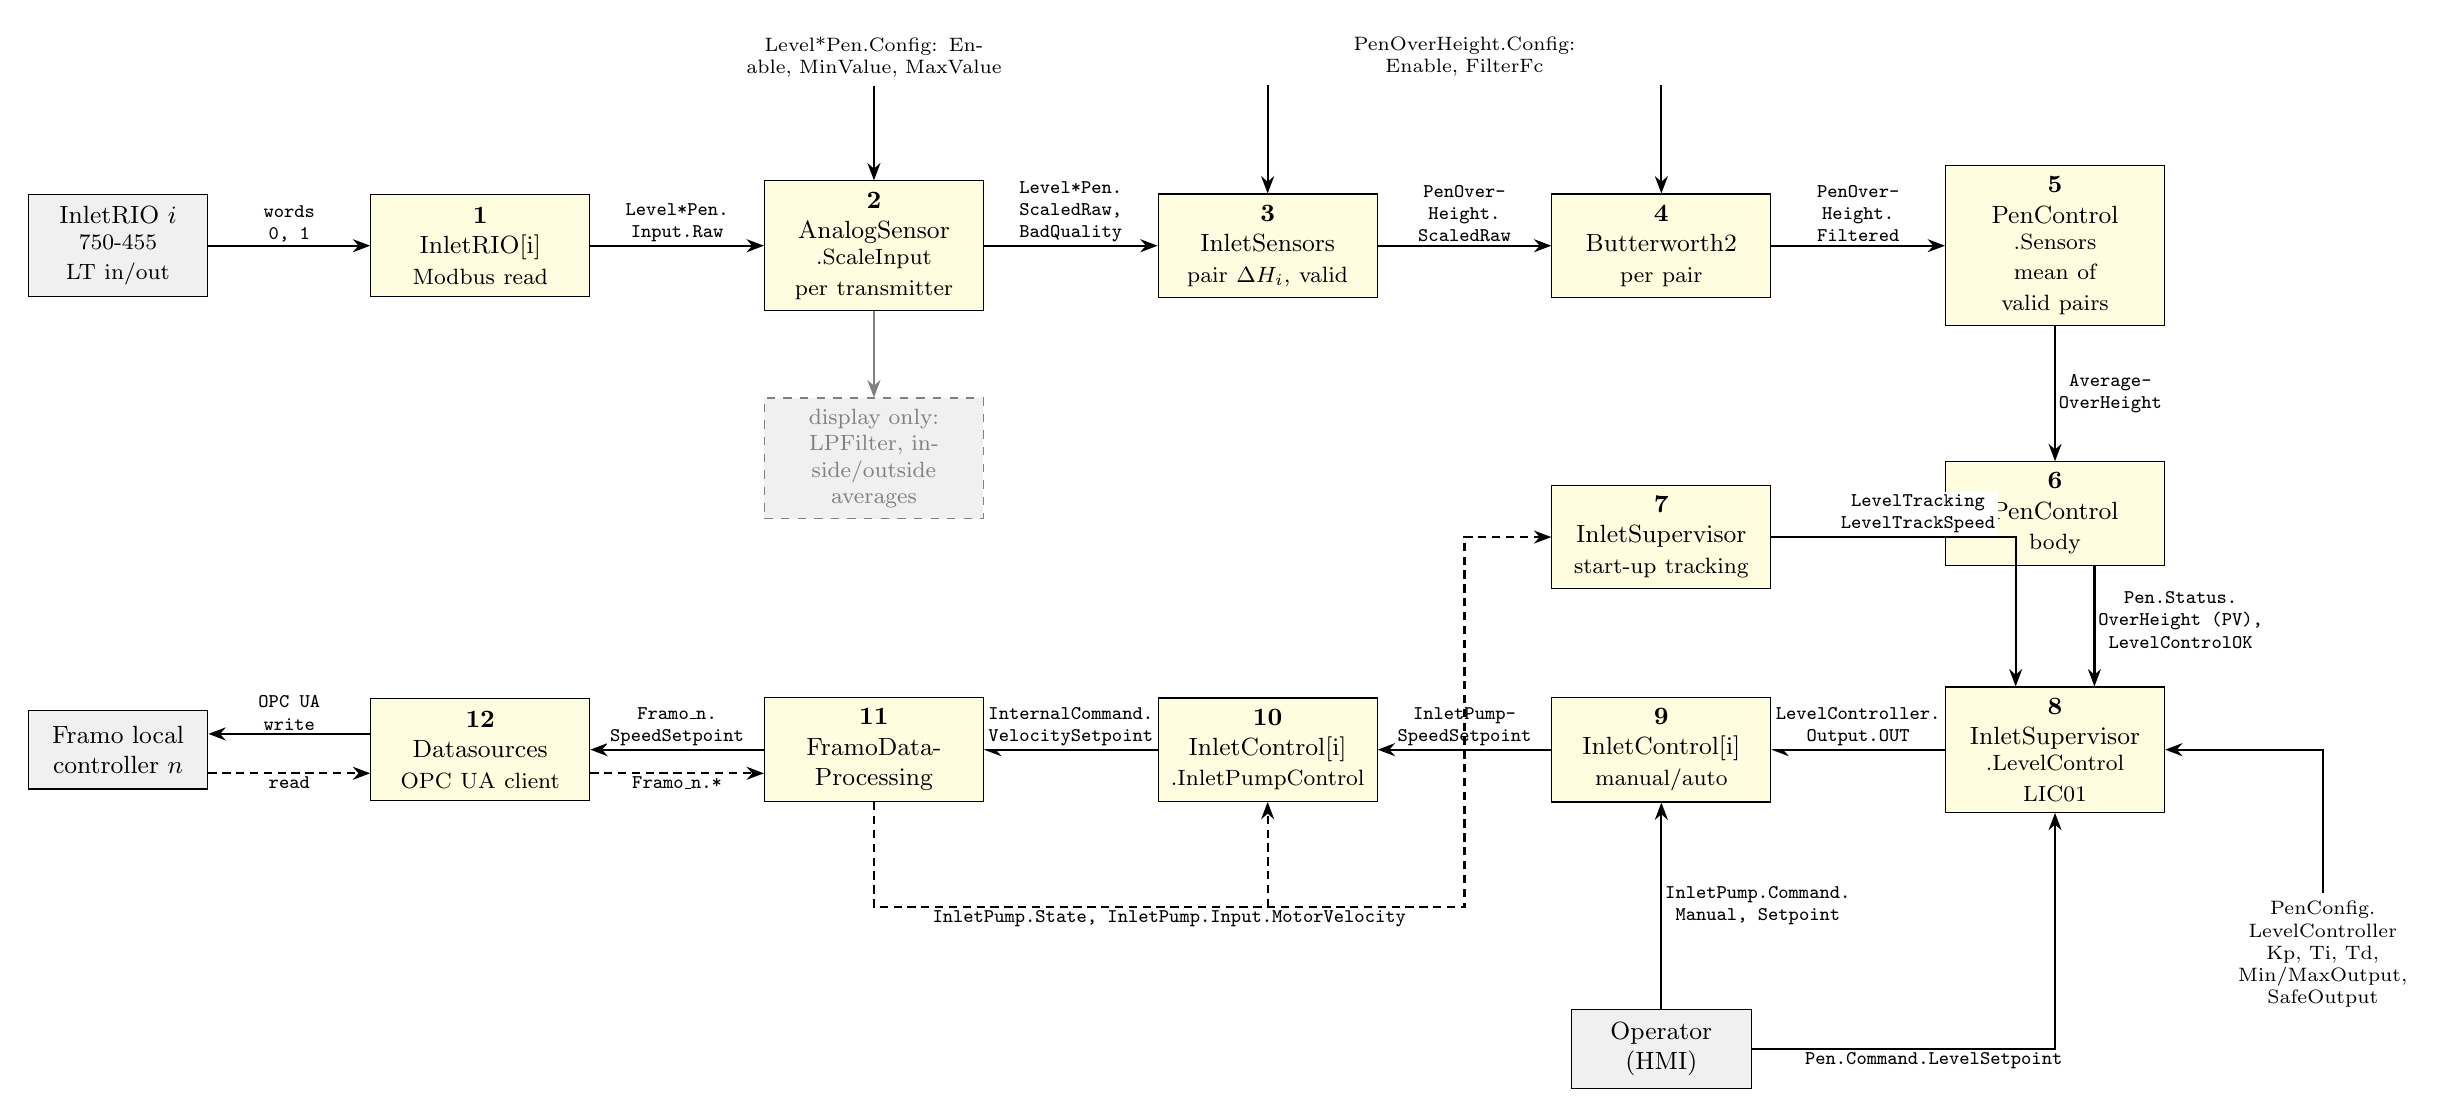
\begin{tikzpicture}[x=10mm, y=10mm, sm/.append style={text width=25mm, minimum height=13mm}]
  % Row A: measurement, left to right
  \node[ext, text width=20mm] (lt) at (0,0) {InletRIO $i$\\\footnotesize 750-455\\\footnotesize LT in/out};
  \node[sm] (s1) at (4.6,0)  {\textbf{1}\\InletRIO[i]\\\footnotesize Modbus read};
  \node[sm] (s2) at (9.6,0)  {\textbf{2}\\AnalogSensor\\\footnotesize .ScaleInput\\\footnotesize per transmitter};
  \node[sm] (s3) at (14.6,0) {\textbf{3}\\InletSensors\\\footnotesize pair $\Delta H_i$, valid};
  \node[sm] (s4) at (19.6,0) {\textbf{4}\\Butterworth2\\\footnotesize per pair};
  \node[sm] (s5) at (24.6,0) {\textbf{5}\\PenControl\\\footnotesize .Sensors\\\footnotesize mean of valid pairs};
  \node[sm] (s6) at (24.6,-3.4) {\textbf{6}\\PenControl\\\footnotesize body};
  \node[extoff, text width=25mm, font=\footnotesize] (disp) at (9.6,-2.7)
       {display only: LPFilter, inside/outside averages};
  \node[store, font=\scriptsize, text width=40mm] (cfgL) at (9.6,2.4)
       {Level*Pen.Config: Enable, MinValue, MaxValue};
  \node[store, font=\scriptsize, text width=48mm] (cfgO) at (17.1,2.4)
       {PenOverHeight.Config: Enable, FilterFc};

  % Row B: control, right to left
  \node[sm] (s7) at (19.6,-3.7) {\textbf{7}\\InletSupervisor\\\footnotesize start-up tracking};
  \node[sm] (s8) at (24.6,-6.4) {\textbf{8}\\InletSupervisor\\\footnotesize .LevelControl\\\footnotesize LIC01};
  \node[sm] (s9) at (19.6,-6.4) {\textbf{9}\\InletControl[i]\\\footnotesize manual/auto};
  \node[sm] (s10) at (14.6,-6.4) {\textbf{10}\\InletControl[i]\\\footnotesize .InletPumpControl};
  \node[sm] (s11) at (9.6,-6.4) {\textbf{11}\\FramoData-\\Processing};
  \node[sm] (s12) at (4.6,-6.4) {\textbf{12}\\Datasources\\\footnotesize OPC UA client};
  \node[ext, text width=20mm] (fr) at (0,-6.4) {Framo local\\controller $n$};

  \node[ext, text width=20mm] (hmi) at (19.6,-10.2) {Operator\\(HMI)};
  \node[store, font=\scriptsize, align=center] (cfgP) at (28.0,-9.0) {PenConfig.\\LevelController\\Kp, Ti, Td,\\Min/MaxOutput,\\SafeOutput};

  % Forward flow
  \draw[flow] (lt) -- node[lab, above] {words\\0, 1} (s1);
  \draw[flow] (s1) -- node[lab, above] {Level*Pen.\\Input.Raw} (s2);
  \draw[flow] (s2) -- node[lab, above] {Level*Pen.\\ScaledRaw,\\BadQuality} (s3);
  \draw[flow] (s3) -- node[lab, above] {PenOver-\\Height.\\ScaledRaw} (s4);
  \draw[flow] (s4) -- node[lab, above] {PenOver-\\Height.\\Filtered} (s5);
  \draw[flow] (s5) -- node[lab, right] {Average-\\OverHeight} (s6);
  \draw[flow, gray] (s2) -- (disp);
  \draw[flow] (cfgL) -- (s2);
  \draw[flow] (cfgO.south -| s3.north) -- (s3.north);
  \draw[flow] (cfgO.south -| s4.north) -- (s4.north);
  \draw[flow] ([xshift=5mm]s6.south) -- node[lab, right, pos=0.45] {Pen.Status.\\OverHeight (PV),\\LevelControlOK} ([xshift=5mm]s8.north);
  \draw[flow] (s7.east) -| node[lab, above, pos=0.3] {LevelTracking\\LevelTrackSpeed} ([xshift=-5mm]s8.north);
  \draw[flow] (s8) -- node[lab, above] {LevelController.\\Output.OUT} (s9);
  \draw[flow] (s9) -- node[lab, above] {InletPump-\\SpeedSetpoint} (s10);
  \draw[flow] (s10) -- node[lab, above] {InternalCommand.\\VelocitySetpoint} (s11);
  \draw[flow] (s11) -- node[lab, above] {Framo\_n.\\SpeedSetpoint} (s12);
  \draw[flow] ([yshift=2mm]s12.west) -- node[lab, above] {OPC UA\\write} ([yshift=2mm]fr.east);

  % Feedback from the pump
  \draw[fb] ([yshift=-3mm]fr.east) -- node[lab, below] {read} ([yshift=-3mm]s12.west);
  \draw[fb] ([yshift=-3mm]s12.east) -- node[lab, below] {Framo\_n.*} ([yshift=-3mm]s11.west);
  \draw[fb] (s11.south) -- (9.6,-8.4) -- node[lab, below] {InletPump.State, InletPump.Input.MotorVelocity} (17.1,-8.4)
        |- (s7.west);
  \draw[fb] (14.6,-8.4) -- (s10.south);

  % Commands and configuration
  \draw[flow] (hmi) -- node[lab, right] {InletPump.Command.\\Manual, Setpoint} (s9);
  \draw[flow] (hmi.east) -| node[lab, below, pos=0.3] {Pen.Command.LevelSetpoint} (s8.south);
  \draw[flow] (cfgP.north) |- (s8.east);
\end{tikzpicture}}
\captionof{figure}{Functional flow diagram of the level loop, one inlet shown [COO Fig.~7.8].
SMs 1--4, 9 and 10 run once per inlet; SMs 5--8 once for the pen. Solid: data flow; dashed:
feedback from the pump. Level*Pen stands for LevelInsidePen and LevelOutsidePen. A pair with a
lost transmitter drops out at SM~3; with no valid pair, SM~8 runs LIC01 at SafeOutput. Execution
order in Figure~\ref{fig:exec}.}
\label{fig:ffd}
\end{center}
\end{landscape}

\begin{landscape}
\small
\begin{longtable}{@{}cP{33mm}P{48mm}P{80mm}P{50mm}@{}}
\caption{Dataflow of the level loop. Unit after each SM in square brackets. ``Main.'' and
``GVLMain.'' prefixes are left out where the context is clear.}
\label{tab:dataflow}\\
\toprule
SM & Code unit (task) & Reads & Operation & Writes \\
\midrule
\endfirsthead
\toprule
SM & Code unit (task) & Reads & Operation & Writes \\
\midrule
\endhead
\bottomrule
\endfoot
1 & \var{IO_Processing.InletRIO[i]} (Task) &
  Modbus TCP response \var{TCPResponse.awData[0..25]} &
  \var{WagoAppPlcModbus.FbMbMasterTcp}, function code 23, reads 26 words from address 0 every
  60~ms (\var{TCPDelay}). \var{InputMapping} copies the words only while
  \var{Status.CommOK}; otherwise the last value stays. &
  \var{GVLMain.Inlet[i].Input.LevelInsidePen.Input.Raw} := word 0;
  \var{GVLMain.Inlet[i].Input.LevelOutsidePen.Input.Raw} := word 1 [counts] \\
2 & \var{InletControl[i].InletSensors.LevelInsidePen.ScaleInput} (Task); same for
  \var{LevelOutsidePen} &
  \var{Input.Raw}, \var{Config.MinValue}, \var{Config.MaxValue} &
  750-455 word: value in bits 14..4, reserved bits 3..2, diagnostics in bits 1..0.
  \code{Quality := Raw AND 2\#11}; \code{Raw := Raw AND 16\#FFF8} (written back to the GVL).\dev{12}
  If \code{Quality = 0}: $\text{ScaledRaw} = \text{Raw}\cdot(\text{Max}-\text{Min})/32760 +
  \text{Min}$, \code{BadQuality := FALSE}; else \code{ScaledRaw := Min},
  \code{BadQuality := TRUE}, and the transmitter's Quality alarm (\var{Config.QualityEnabled},
  1~s). The per-transmitter \var{LPFilter} (\var{SCL.Butterworth}) gives \var{.Filtered} for
  display only. &
  \var{Inlet[i].Input.LevelInsidePen.ScaledRaw} [m], \var{.Status.BadQuality} \\
3 & \var{InletControl[i].InletSensors} (Task) &
  \var{LevelInsidePen.ScaledRaw}, \var{LevelOutsidePen.ScaledRaw}, their \var{.Config.Enable} and
  \var{.Status.BadQuality}, \var{PenOverHeight.Config.Enable} &
  Level pair of the inlet [FD \S3.2.2]: $\Delta H_i$ = inside $-$ outside from the unfiltered
  scaled values. The pair is valid when both transmitters are enabled and healthy and the pair is
  enabled; if either transmitter is lost, the whole pair drops out. &
  \var{Inlet[i].Input.PenOverHeight.ScaledRaw} [m], \var{.Status.BadQuality} (= not valid) \\
4 & \var{InletSensors.OverHeightFilter} (\var{Butterworth2}) (Task) &
  \var{PenOverHeight.ScaledRaw}, \var{PenOverHeight.Config.FilterFc} &
  Second-order Butterworth low-pass on the pair's $\Delta H_i$, LREAL, bilinear with
  pre-warping. Sample time: the calling task's cycle time (\var{GetTaskIntervalUs},
  \var{CmpIecTask}). Restarts at the current value when
  the pair becomes valid (and at start), so a returning pair causes no dip. &
  \var{Inlet[i].Input.PenOverHeight.Filtered} [m] (0 while not valid) \\
5 & \var{PenControl.Sensors} (Task) &
  \var{Inlet[0..2].Input.PenOverHeight.Filtered}, \var{.Status.BadQuality} &
  Mean of the filtered $\Delta H_i$ of the valid pairs. Bad when no pair is valid. (The mean
  inside and outside levels are computed alongside, for display.) &
  \var{Pen.Input.AverageOverHeight.Filtered} [m], \var{.Status.BadQuality} \\
6 & \var{PenControl} body and \var{.AlarmHandling} (Task) &
  \var{Pen.Input.AverageOverHeight} &
  Process value of LIC01, and \code{LevelControlOK := NOT BadQuality}. Alarm
  \var{Pen.Alarm.LevelMeasurementLost} while no pair is valid. &
  \var{Pen.Status.OverHeight} [m], \var{Pen.Status.LevelControlOK} \\
7 & \var{InletSupervisor} body (Task) &
  \var{Inlet[i].InletPump.State}, \var{.Status.EnableLevelControl},
  \var{.Input.MotorVelocity} &
  Start-up tracking [FD \S3.2.1]: if a pump in level control is in START and none is in REMOTE,
  \code{LevelTracking := TRUE} and \var{LevelTrackSpeed} = mean actual speed of the starting
  pumps. Heartbeat loss [FD Tabell~5]: \code{LevelHold} while a pump that was in level control
  has no link or is in HOLD (output frozen at \var{LevelHoldOutput}); then \code{LevelResume} for
  one LIC01 cycle on the mean actual speed of the pumps in level control. &
  \var{LevelTracking}, \var{LevelTrackSpeed}, \var{LevelHold}, \var{LevelResume} [rpm] (local) \\
8 & \var{InletSupervisor.LevelControl} (\var{PIDController}) $\to$ \var{Util.PID} (Task) &
  SP \var{Pen.Command.LevelSetpoint}, PV \var{Pen.Status.OverHeight},
  \var{Pen.Status.LevelControlOK}, \var{PenConfig.LevelController.*},
  \var{LevelController.Command.*}, SM~7 &
  Enabled when \var{PenStart} and at least one pump in level control. Manual when the operator
  says so, when the level is lost (\code{NOT LevelControlOK}), on heartbeat loss (hold, resume) or
  while tracking; the manual output is, in that order, the operator's, \var{SafeOutput} (limited
  to Min/MaxOutput), the frozen output, the resume speed or \var{LevelTrackSpeed}.
  PI: $Y = K_p\,(e + \tfrac{1}{T_i}\int e\,dt + T_d\,\dot e) + Y_\text{offset}$, limited to
  \var{MinOutput..MaxOutput}. Manual$\to$auto: \var{RESET} with
  $Y_\text{offset} = Y_\text{prev} - K_p e$ (bumpless). &
  \var{GVLMain.LevelController.Output.OUT} [rpm],
  \var{LevelController.Input.LimitsActive}, \var{.Overflow} \\
9 & \var{Main} $\to$ \var{InletControl[i]} body (Task) &
  \var{LevelControllerOut} := \var{GVLMain.LevelController.Output.OUT},
  \var{InletPump.Status.Manual}, \var{InletPump.Command.Setpoint} &
  \code{InletPumpSpeedSetpoint := Command.Setpoint} in manual, \var{LevelControllerOut} in auto.
  One setpoint for all pumps in auto [FD \S3.2.2]. &
  \var{InletPumpSpeedSetpoint} [rpm] (local) \\
10 & \var{InletControl[i].InletPumpControl} (Task) &
  \var{AutoSpeedSetpoint} (= SM~9), \var{InletPump.State}, \var{InletPump.Input.MotorVelocity} &
  Per state (Table~\ref{tab:states}): REMOTE sends the setpoint; AVAILABLE, START and HOLD send the
  actual speed; the other states 0. Body: \code{InternalCommand.VelocitySetpoint :=
  Output.VelocitySetpoint}. Also sets \var{Status.EnableLevelControl}, \var{Status.ActualSpeed}. &
  \var{Inlet[i].InletPump.Output.VelocitySetpoint},
  \var{Inlet[i].InletPump.InternalCommand.VelocitySetpoint} [rpm] \\
11 & \var{FramoDataProcessing} (OPC\_Processing) &
  \var{Inlet[i].InletPump.InternalCommand.VelocitySetpoint}; \var{Framo_n.*} &
  Out: \code{Framo\_n.SpeedSetpoint.Value := VelocitySetpoint} (REAL$\to$LREAL). In:
  \code{InletPump.Input.MotorVelocity := LREAL\_TO\_REAL(Framo\_n.MotorVelocity.Value)}, alarms,
  heartbeat, state (Table~\ref{tab:startflow}, F). &
  \var{Framo_n.SpeedSetpoint.Value} [rpm]; \var{Inlet[i].InletPump.Input.*},
  \var{Inlet[i].InletPump.State} \\
12 & \var{Datasources_PRG} (DatasourcesTask) &
  data source variables \var{Framo_n} &
  OPC UA client: writes \var{SpeedSetpoint}, \var{Start}, \var{Stop}, \var{Reset} to the Framo
  controller's nodes (\var{VelocitySetpoint} etc.\ in [FD Tabell~6]) and reads its variables. &
  Framo controller $n$ \\
\end{longtable}
\end{landscape}

% ---------------------------------------------------------------------------------------------
\begin{landscape}
\section{Oxygen system}
\label{sec:oxygen}

The oxygen system follows the cascade of [FD \S3.2.4]: OIC01 on the pen O$_2$ over one flow loop
(FIC) per line, with the oxy pump of each line on a pressure loop (PIC). OIC01's output is the
\emph{total} O$_2$ flow to the pen, shared between the lines in auto (SM~O3). Figure~\ref{fig:oxyffd}
is the functional flow diagram, Table~\ref{tab:oxyflow} the dataflow. All SMs run in \var{Task}:
O1 in \var{PenControl}, O2--O3 in \var{InletSupervisor}, O4--O9 in \var{OxyControl[i]}, O10 in
\var{IO_Processing}.

\begin{center}
\resizebox{\linewidth}{!}{%
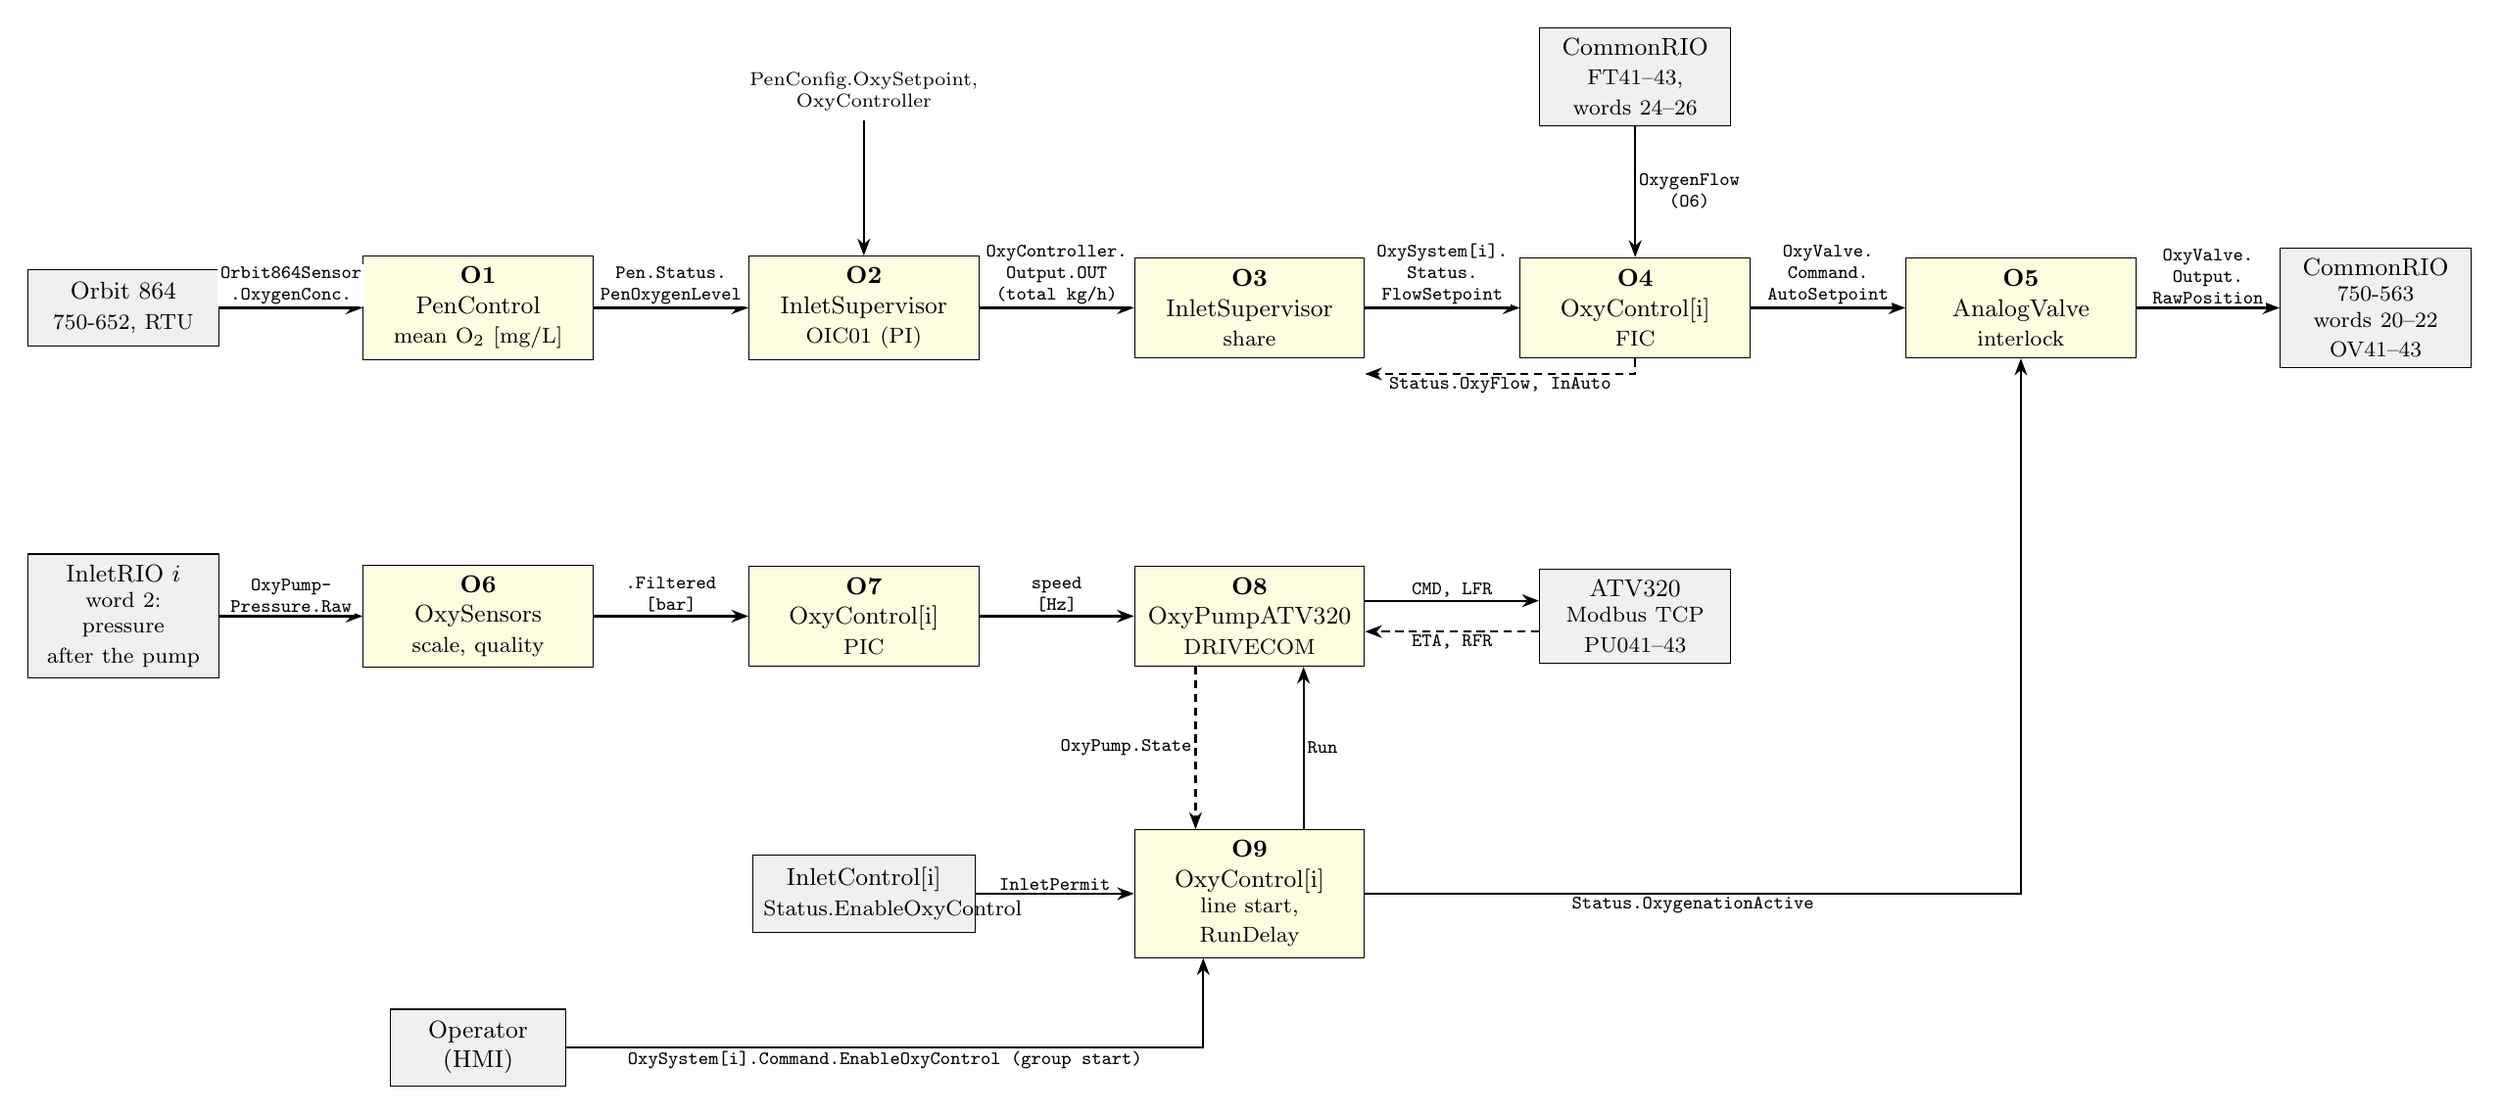
\begin{tikzpicture}[x=10mm, y=10mm, sm/.append style={text width=27mm, minimum height=13mm}]
  % Row A: O2 measurement and OIC01
  \node[ext, text width=22mm] (ot) at (0,0) {Orbit 864\\\footnotesize 750-652, RTU};
  \node[sm] (o1) at (4.6,0) {\textbf{O1}\\PenControl\\\footnotesize mean O$_2$ [mg/L]};
  \node[sm] (o2) at (9.6,0) {\textbf{O2}\\InletSupervisor\\\footnotesize OIC01 (PI)};
  \node[sm] (o3) at (14.6,0) {\textbf{O3}\\InletSupervisor\\\footnotesize share};
  \node[sm] (o4) at (19.6,0) {\textbf{O4}\\OxyControl[i]\\\footnotesize FIC};
  \node[sm] (o5) at (24.6,0) {\textbf{O5}\\AnalogValve\\\footnotesize interlock};
  \node[ext, text width=22mm] (crio) at (29.2,0) {CommonRIO\\\footnotesize 750-563 words 20--22\\\footnotesize OV41--43};
  \node[ext, text width=22mm] (ft) at (19.6,3.0) {CommonRIO\\\footnotesize FT41--43, words 24--26};
  \node[store, font=\scriptsize, align=center] (cfgO) at (9.6,2.8) {PenConfig.OxySetpoint,\\OxyController};

  % Row B: pump and permissive
  \node[ext, text width=22mm] (irio) at (0,-4.0) {InletRIO $i$\\\footnotesize word 2: pressure\\\footnotesize after the pump};
  \node[sm] (o6) at (4.6,-4.0) {\textbf{O6}\\OxySensors\\\footnotesize scale, quality};
  \node[sm] (o7) at (9.6,-4.0) {\textbf{O7}\\OxyControl[i]\\\footnotesize PIC};
  \node[sm] (o8) at (14.6,-4.0) {\textbf{O8}\\OxyPumpATV320\\\footnotesize DRIVECOM};
  \node[ext, text width=22mm] (atv) at (19.6,-4.0) {ATV320\\\footnotesize Modbus TCP\\\footnotesize PU041--43};
  \node[sm] (o9) at (14.6,-7.6) {\textbf{O9}\\OxyControl[i]\\\footnotesize line start,\\\footnotesize RunDelay};
  \node[ext, text width=26mm] (inl) at (9.6,-7.6) {InletControl[i]\\\footnotesize Status.EnableOxyControl};
  \node[ext, text width=20mm] (hmi) at (4.6,-9.6) {Operator\\(HMI)};

  % flows row A
  \draw[flow] (ot) -- node[lab, above] {Orbit864Sensor\\.OxygenConc.} (o1);
  \draw[flow] (o1) -- node[lab, above] {Pen.Status.\\PenOxygenLevel} (o2);
  \draw[flow] (cfgO) -- (o2);
  \draw[flow] (o2) -- node[lab, above] {OxyController.\\Output.OUT\\(total kg/h)} (o3);
  \draw[flow] (o3) -- node[lab, above] {OxySystem[i].\\Status.\\FlowSetpoint} (o4);
  \draw[flow] (o4) -- node[lab, above] {OxyValve.\\Command.\\AutoSetpoint} (o5);
  \draw[flow] (o5) -- node[lab, above] {OxyValve.\\Output.\\RawPosition} (crio);
  \draw[flow] (ft) -- node[lab, right] {OxygenFlow\\(O6)} (o4);
  \draw[fb] (o4.south) |- node[lab, pos=0.75, below] {Status.OxyFlow, InAuto} ([yshift=-2mm]o3.south east) ;

  % flows row B
  \draw[flow] (irio) -- node[lab, above] {OxyPump-\\Pressure.Raw} (o6);
  \draw[flow] (o6) -- node[lab, above] {.Filtered\\{[bar]}} (o7);
  \draw[flow] (o7) -- node[lab, above] {speed\\{[Hz]}} (o8);
  \draw[flow] ([yshift=2mm]o8.east) -- node[lab, above] {CMD, LFR} ([yshift=2mm]atv.west);
  \draw[fb] ([yshift=-2mm]atv.west) -- node[lab, below] {ETA, RFR} ([yshift=-2mm]o8.east);
  \draw[flow] (hmi.east) -| node[lab, pos=0.25, below] {OxySystem[i].Command.EnableOxyControl (group start)} ([xshift=-6mm]o9.south);
  \draw[flow] (inl) -- node[lab, above] {InletPermit} (o9);
  \draw[fb] ([xshift=-7mm]o8.south) -- node[lab, left] {OxyPump.State} ([xshift=-7mm]o9.north);
  \draw[flow] ([xshift=7mm]o9.north) -- node[lab, right] {Run} ([xshift=7mm]o8.south);
  \draw[flow] (o9.east) -| node[lab, pos=0.25, below] {Status.OxygenationActive} (o5.south);
\end{tikzpicture}}
\captionof{figure}{Functional flow diagram of the oxygen system [COO Fig.~7.8]; one line shown for
O4--O9. Solid: data flow; dashed: feedback.}
\label{fig:oxyffd}
\end{center}
\end{landscape}

\begin{landscape}
\small
\begin{longtable}{@{}cP{33mm}P{50mm}P{82mm}P{48mm}@{}}
\caption{Dataflow of the oxygen system.}\label{tab:oxyflow}\\
\toprule
SM & Code unit & Reads & Operation & Writes \\
\midrule
\endfirsthead
\toprule
SM & Code unit & Reads & Operation & Writes \\
\midrule
\endhead
\bottomrule
\endfoot
O1 & \var{PenControl.Sensors}, body &
  \var{Pen.Input.Orbit864Sensor[0..5].OxygenConcentration} &
  Mean of the sensors marked for control and in good quality; bad when none is good. &
  \var{Pen.Status.PenOxygenLevel} [mg/L], \var{Pen.Status.OxyControlOK} \\
O2 & \var{InletSupervisor.OxyControl} (\var{PIDController}) &
  SP \var{PenConfig.OxySetpoint}, PV O1, \var{PenConfig.OxyController}, the lines' status &
  PI to the total O$_2$ flow [kg/h]. Enabled with \var{PenStart} and at least one line in auto.
  Limited to what the lines in auto can deliver plus the manual lines' flow. Manual: operator;
  frozen while \code{NOT OxyControlOK}; first enabled cycle from the measured total flow
  (bumpless). &
  \var{OxyController.Output.OUT} [kg/h] \\
O3 & \var{InletSupervisor} &
  O2, \var{OxySystem[i].Status.InAuto}, \var{.OxyFlow}, \var{OxyConfig[i].FlowMax} &
  Share: (total $-$ measured flow of the active lines not in auto) / number of lines in auto,
  each limited to its \var{FlowMax}. A lost line or a moved manual line is made up at once. &
  \var{OxySystem[i].Status.FlowSetpoint} [kg/h] \\
O4 & \var{OxyControl[i].FlowControl} (FIC) &
  SP O3, PV \var{Status.OxyFlow} (FT, 0--150 kg/h) &
  PI to the valve position 0--100 \%. In auto when oxygenation is active, the valve in auto and
  the flow good; manual output 0 (not active), the operator's valve position, or held. &
  \var{OxyValve.Command.AutoSetpoint} [\%], \var{Status.InAuto} \\
O5 & \var{OxyControl[i].OxyValveControl} (\var{AnalogValve}) &
  \var{OxyValve.Command}, \var{Status.OxygenationActive} &
  Setpoint (auto or manual) to 0--65535 for the 750-563 (4--20 mA). Forced to 0 (closed) unless
  oxygenation is active. &
  \var{OxySystem[i].OxyValve.Output.RawPosition} $\to$ CommonRIO word 20+i \\
O6 & \var{OxyControl[i].OxySensors} &
  InletRIO word 2/3, CommonRIO word 24+i &
  Scale and health check (\var{AnalogSensor}) of the pressure after the pump, after the
  oxygenator, and the O$_2$ flow. &
  \var{OxySystem[i].Input.*.Filtered} \\
O7 & \var{OxyControl[i].PressureControl} (PIC) &
  SP \var{Config.PressureSetpoint} (4.0 bar), PV pressure after the pump &
  PI to the pump speed, \var{MinSpeed_Hz..MaxSpeed_Hz}. Preset speed while starting, in pump
  manual (operator speed), with \var{PressureController.Enabled} off or a bad pressure. &
  speed setpoint [Hz] \\
O8 & \var{OxyControl[i].Drive} (\var{OxyPumpATV320}) &
  Run (O9), speed, \var{OxyPump.Command.Reset}, \var{Config.OxyPump} (IP, port, unit id) &
  Modbus TCP every 100 ms, FC23: write CMD 8501, LFR 8502 (0.1 Hz); read 3201--3211 (ETA, RFR,
  LCR, THD, OPR), every 10th request LFT 7121. DRIVECOM: 0x0006, 0x0007, 0x000F to run, 0x0007 to
  stop, 0x0080 to reset a fault. Pump state from ETA and speed. &
  \var{OxyPump.Input.*}, \var{OxyPump.State}, \var{OxyPump.Status.CommunicationOK} \\
O9 & \var{OxyControl[i]} body, \var{.OxyPumpControl} &
  \var{Command.EnableOxyControl}, \var{InletPermit}, \var{OxyPump.State}, \var{.Status.Manual} &
  Line started = operator's group start AND the inlet pump in REMOTE with a live link (D3). Auto:
  the oxy pump runs while the line is started; manual: \var{OxyPump.Command.Start/Stop}.
  Oxygenation active after the pump has run \var{Config.OxyPump.RunDelay}. &
  Run, \var{Status.OxygenationActive} \\
O10 & \var{IO_Processing.CommonRIO} &
  \var{GVLMain.OxySystem[i].OxyValve} &
  Output mapping to CommonRIO words 20--22. &
  Modbus TCP to the CommonRIO \\
\end{longtable}
\end{landscape}

\subsection*{Oxygen configuration and commands}

\begin{table}[htbp]
\centering\small
\caption{Configuration of the oxygen system, retained (\texttt{GVLRetain}), defaults from
\texttt{PFC200\_Sim} \texttt{ConfigValues}. Tuning values are start values for commissioning.}
\label{tab:oxyconfig}
\begin{tabularx}{\textwidth}{@{}P{62mm}P{36mm}L@{}}
\toprule
Variable & Default & Meaning \\
\midrule
\var{PenConfig.OxySetpoint} & 8.0 mg/L & OIC01 setpoint (placeholder until [FD] gives it). \\
\var{PenConfig.OxyController} & $K_p$ 50, $T_i$ 1800 s & OIC01, (kg/h)/(mg/L); \var{MaxOutput} 0 = what the lines can deliver. \\
\var{OxyConfig[i].OxyPump.IP}, \var{.Port}, \var{.UnitId}, \var{.Enable} & 10.1.2.101, 5131--5133, 0, TRUE & ATV320 of line $i$ (simulator on the test rig). \\
\var{OxyConfig[i].OxyPump.Min/MaxSpeed_Hz}, \var{.PresetSpeed_Hz} & 20, 50, 40 Hz & PIC output range; speed while starting or in manual. \\
\var{OxyConfig[i].OxyPump.RunDelay} & 30 s & Pump at speed this long before oxygen is added. \\
\var{OxyConfig[i].PressureController}, \var{.PressureSetpoint} & $K_p$ 2 Hz/bar, $T_i$ 5 s; 4.0 bar & PIC; \var{Enabled} FALSE runs the preset speed. \\
\var{OxyConfig[i].FlowController}, \var{.FlowMax} & $K_p$ 0.3 \%/(kg/h), $T_i$ 5 s; 104.2 kg/h & FIC; most flow of the line. \\
\var{OxyConfig[i].OxyStartupTime}, \var{.OxyShutdownTime} & 10 s, 10 s & Drive start (not turning) and stop (still turning) alarms. \\
\var{GVLRetain.OxyPumpPressureConfig[i]}, \var{OxynatorOutletPressureConfig[i]}, \var{OxygenFlowConfig[i]} & 0--10 bar, 0--10 bar, 0--150 kg/h & Sensor ranges, filters, quality alarms. \\
\bottomrule
\end{tabularx}
\end{table}

Commands: \var{OxySystem[i].Command.EnableOxyControl} starts and stops line $i$ (group start);
\var{OxySystem[i].OxyPump.Command.Manual/Auto/Start/Stop/Reset/Setpoint} run the oxy pump by hand;
\var{OxySystem[i].OxyValve.Command.Manual/ManualSetpoint} hold the valve by hand (the line then
counts as manual in O3); \var{OxyController.Command.Manual/ManualOutput} hold OIC01's total flow.

% ---------------------------------------------------------------------------------------------
\section{Deviations and open issues}
\label{sec:dev}

Found while tracing the dataflow and comparing it with [FD]. The marks \dev{n} in the tables refer
to this list.

\begin{longtable}{@{}lP{66mm}P{80mm}@{}}
\toprule
& Finding & Consequence / suggestion \\
\midrule
\endhead
\bottomrule
\endfoot
D1 & \textbf{Heartbeat not wired.} \var{InletControl.Heartbeat} watches the local
  \var{HeartbeatToggle}, which is never written; \var{FramoDataProcessing} writes
  \var{InletPump.Input.HeartbeatToggle}. [FD \S3.2.1] &
  \var{HeartbeatTimeout} is TRUE after 1~s and stays TRUE: the communication alarm is
  permanent and a real link loss is not detected. \textbf{Fixed} 2026-10-15 (in review): one
  shared bit \var{Framo_n.HeartbeatToggle}, the PLC sets it while FALSE (after
  \var{InletConfig.HeartbeatInterval}), Framo clears it while TRUE; alarm when Framo has not cleared
  it for \var{InletConfig.HeartbeatTimeout}. CasFramoSim implements Framo's half; the simulator UI
  injects \emph{Heartbeat lost}. \\
D2 & \var{DriveError} alarm wrote \var{InletPump.Alarm.DriveNotInRemote}. &
  \textbf{Fixed} 2026-10-15 (in review): it writes \var{Alarm.DriveError}. \\
D3 & \textbf{HOLD.} [FD Tabell~5]: on heartbeat loss the LIC01 output shall freeze and, when the
  link is back, start from the actual pump speed. Oxygenation in that line shall stop. &
  \textbf{Fixed} 2026-10-15 (in review). \var{InletSupervisor}: when the link to a pump that was in
  level control is lost, LIC01 is frozen at its output; it stays frozen while the link is down and,
  once back, while the pump is in HOLD (the operator resets it). When the pump is in REMOTE again (or
  no longer running), LIC01 runs one cycle on the mean actual speed of the pumps in level control and
  returns to auto bumplessly. \var{InletControl} sets \var{Status.EnableOxyControl} only with a live
  link and the pump in REMOTE: the permissive for the oxygen system on that line. \\
D4 & \textbf{Process value.} [FD \S3.2.2]: mean of the per-inlet $\Delta H_i$ of the active
  pairs. Code was: mean of all good inside minus mean of all good outside transmitters. &
  \textbf{Fixed} 2026-10-15 (in review): $\Delta H_i$ per pair, filtered per pair
  (\var{Butterworth2}), mean of the valid pairs; a lost transmitter drops its whole pair (SM~3--5). \\
D5 & LIC01 did not check \var{Pen.Input.AverageOverHeight.Status.BadQuality}. &
  With all transmitters bad the PV was $0$~m and LIC01 drove the pumps to \var{MaxOutput}.
  \textbf{Fixed} 2026-10-15 (in review): the health check uses status bits 1..0 only; with no valid
  pair, alarm \emph{LevelMeasurementLost} and LIC01 in manual at \var{SafeOutput} (60~rpm),
  bumpless back to auto. \\
D6 & [FD Tabell~8]: one parameter set per number of running pumps. & One set only (known, deferred). \\
D7 & [FD Tabell~7]: alarm on speed deviation in REMOTE. & Not implemented. \\
D8 & [FD Tabell~7]: start alarm if the pump does not report START within a preset time after the
  start command. & Code measured the time \emph{in} START, so a pump that never left AVAILABLE gave
  no alarm, and a normal START sequence longer than 30~s did. \textbf{Fixed} 2026-10-15 (in review):
  \var{StartupTransitionTimer} runs while Start is commanded and the pump is still AVAILABLE;
  \var{ShutdownTransitionTimer} while Stop is commanded and the pump is still starting, in REMOTE or
  in HOLD. Framo's own START and STOP sequences are not timed. \\
D9 & \var{ENUM.InletPumpState} has \code{Available := 0}, and \var{FramoDataProcessing} only
  writes the state when one of the flags is TRUE. &
  With no OPC UA data the PLC saw AVAILABLE and allowed \var{Start}. \textbf{Fixed} 2026-10-15
  (in review): \var{InletControl} sets \var{Status.CommunicationOK} once Framo has answered the
  heartbeat (cleared until the timeout); without it \var{FramoDataProcessing} reports UNAVAILABLE. \\
D10 & \var{AnalogSensor.TaskIntervalUs} was a constant 10\,000~µs. &
  \textbf{Fixed} 2026-10-15 (in review): \var{GetTaskIntervalUs} reads the cycle time of the calling
  task from the runtime (\var{CmpIecTask}: \var{IecTaskGetCurrent}, \var{IecTaskGetInfo3}).
  \var{AnalogSensor} and \var{Butterworth2} read it once; fallback 10~ms (\var{AnalogSensor}) or the
  measured call interval (\var{Butterworth2}) if the runtime gives none (event task). All filter
  instances are called from \var{Main} in \var{Task}. \\
D11 & \var{ConfigValues} had \code{PenConfig.LevelController.Ti := 600}, the [FD] start value. The
  site test used 60~s [DES \S7]. & \textbf{Fixed} 2026-10-15 (in review): \code{Ti := 60} in
  \var{PFC200_Sim} \var{ConfigValues}. Applies on a fresh download; check the retained value. \\
D12 & \var{AnalogSensor.Input} was \var{VAR_IN_OUT}; \var{ScaleInput} wrote the masked word back. &
  \textbf{Fixed} 2026-10-15 (in review): \var{ScaleInput} takes \var{Input} as a \var{VAR_INPUT}
  copy; \var{Input.Raw} keeps the status bits for the HMI. \\
D13 & \var{Pen.Command.LevelSetpoint} was not retained. [FD]: setpoint from the operating mode of
  the outlet valve (HOLD). & \textbf{Fixed} 2026-10-15 (in review): \var{GVLRetain.LevelSetpoint},
  kept in step by \var{Main.UpdateRetain}; default 0.06~m. \\
D14 & \var{PRG.Controllers} (LIC01, oxygen and oxy pump PIDs) was not called by \var{PFC200_Sim}. &
  \textbf{Removed} 2026-10-15 (in review). The legacy application \var{ControlWinSim} still has a
  \var{Controllers} task for it, to be updated. \\
D15 & \var{InletRIO.InputMapping} had \code{MainCircuitBreakerTripped := InputData[2].2},
  \code{BackupPowerOn := InputData[3].3}. Words 2 and 3 are analog (pressures). &
  \textbf{Fixed} 2026-10-15 (in review): \var{InputData[4].2} and \var{InputData[4].3}, next to the
  other word-4 power bits (as the simulator). To confirm against the cabinet drawings. \\
\end{longtable}

\end{document}
